\documentclass{article}
\usepackage{tikz}
\usetikzlibrary{arrows.meta}

\begin{document}

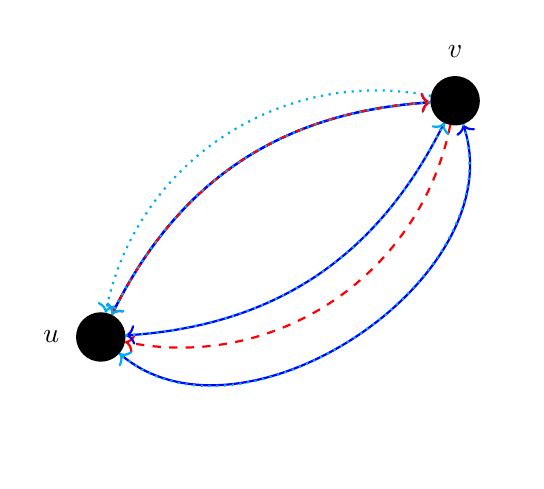
\begin{tikzpicture}[scale=1.5, every node/.style={circle, draw=black!100, thick, minimum size=6mm, inner sep=2pt}]
    \node (v) at (0, 0) [label=above:$v$, fill=black] {};
    \node (u) at (-3, -2) [label=left:$u$, fill=black] {};

    % Draw edges with different colors and styles
    \draw[red, dashed, thick, ->] (v) edge[bend left=45] (u);
    \draw[cyan, dotted, thick, ->] (v) edge[bend right=45] (u);
    \draw[blue, solid, thick, ->] (v) edge[bend left] (u);
    \draw[blue, solid, thick, ->] (u) edge[bend left] (v);
    \draw[blue, solid, thick, ->] (v) edge[bend right] (u);
    \draw[cyan, dotted, thick, ->] (u) edge[bend right] (v);
    \draw[blue, solid, thick, ->] (u) edge[bend right=75] (v);
    \draw[cyan, dotted, thick, ->] (v) edge[bend left=75] (u);
    
    % Connect corner nodes
    \draw[red, dashed, thick, ->] (u) edge[bend left] (v);
    \draw[cyan, dotted, thick, ->] (v) edge[bend right] (u);
\end{tikzpicture}

\end{document}